\chapter{Requirement analysis}\label{chapter:requirements}

%%%%%%%%%%%%%%%%%%%%%%%%%%%%%%%%%%%%%%%%%%%%%%%%%%%%%%%%%%%%%%%%%%%%%%%%%%%%%%%%%%%%%%%%%%%%%%%%%%%
%%%%%%%%%%%%%%%%%%%%%%											USER PROFILE											%%%%%%%%%%%%%%%%%%%%%
%%%%%%%%%%%%%%%%%%%%%%%%%%%%%%%%%%%%%%%%%%%%%%%%%%%%%%%%%%%%%%%%%%%%%%%%%%%%%%%%%%%%%%%%%%%%%%%%%%%
\section{User profile}

The target audience of the application includes users that look for new music or artists based on generated recommendations. In \cite{song:2012}, a classification of music listeners is given. This classification by Jennings categorizes users, aged $16$-$45$, in one of four groups, as listed in table \ref{table:jennings:listeners}.


\begin{table}[h]
\caption{Categorization of music listeners by Jennings, adapted from \cite{song:2012}.}
\begin{center}
	\begin{tabular}{ l | r | p{250px} } % l = left-aligned column
		\hline
		\textbf{Type}			&		\textbf{Percentage}			&			\textbf{Features} \\
		\hline
		Savants 			& $7$		& Everything in life seems to be tied up with music. Their musical knowledge is extensive. \\
		Enthousiasts 	& $21$	& Music is a key part of life but is also balanced by other interests. \\
		Casuals				& $32$	& Music plays a welcome role, but other things are far more important. \\
		Indifferents	& $40$	& They would not loose much sleep if music ceased to exist, they are a predominant type of listeners of the whole population. \\
		\hline
	\end{tabular}
\end{center}
\label{table:jennings:listeners}
\end{table}

It is clear that indifferents are likely to have little interest in receiving particular artist recommendations, let alone finding out how the recommendations were computed. The focus of the application is mainly on enthousiasts and savants, as these users are more likely to look actively for music. These listeners are also more likely to look for music down the \emph{tail}\cite{song:2012}, cf. section \ref{chapter:literature_study:section:computer}.

Table \ref{tab:user_profile1} tries to establish a profile of the target users. Note that most of this user profile is what we expect the application's users to be like, rather than the result of surveys or other types of investigation.

\begin{table}[h]
\caption{User profile 1: sketching the targeted audience}
\begin{center}
	\begin{tabular}{ l p{300px} } % l = left-aligned column
		\hline
		\textbf{Skill set:}		& $*$ Has basic knowledge of computers; \\
													& $*$ Uses mouse for navigation and keyboard for entering text;	\\
													& $*$ Is familiar with traditional website layouts;	\\
													& $*$ Has basic proficiency in English;	\\
		
		\textbf{Behaviour:}		& $*$ Pays regular visits to sites like or similar to \emph{Last.fm}, \emph{IMDb.com}, \emph{netflix.com}, \emph{YouTube.com}, and \emph{amazon.com} and has an account on one or more of these websites; \\
													& $*$ Uses applications such as \emph{iTunes}, \emph{Windows Media Player}, and \emph{Spotify} to listen to and purchase music; \\
													& $*$ Has used recommender systems before. \\
		
		\textbf{Interests:}		& Can be classified as a music enthousiast or savant. \\
		\textbf{Demography:}	& $*$ Aged between 16 and 45 years old;	\\
													& $*$ Both male and female users.	\\
		
		\hline
	\end{tabular}
\end{center}
\label{tab:user_profile1}
\end{table}


User goals with a relevant a part of the application's functionality are the following:

\begin{itemize}
	\item The user wants suggestions, filtering out possibly interesting items from the vast item space. \textit{Suggestions are listed by the system, based on the user's interests. The user can add suggestions to his/her profile.}
	\item The user wants to gain insight into the reasoning behind the suggestions. \textit{Through the explanation system, the underlying conceptual model is visualized.}
	\item The user wants an indication of how reliable the suggestion is. \textit{By providing contextual information for each recommendation, the user can estimate how well the recommendation corresponds to his/her profile.}
\end{itemize}



%%%%%%%%%%%%%%%%%%%%%%%%%%%%%%%%%%%%%%%%%%%%%%%%%%%%%%%%%%%%%%%%%%%%%%%%%%%%%%%%%%%%%%%%%%%%%%%%%%%
%%%%%%%%%%%%%%%%%%%%%%											STORY (BOARD) 										%%%%%%%%%%%%%%%%%%%%%
%%%%%%%%%%%%%%%%%%%%%%%%%%%%%%%%%%%%%%%%%%%%%%%%%%%%%%%%%%%%%%%%%%%%%%%%%%%%%%%%%%%%%%%%%%%%%%%%%%%

\section{User story}

The following user story tries to establish a context in which the application might prove useful. It build on the target audience, defined earlier in table \ref{tab:user_profile1}.

\textit{Imagine you have a music library with a number of tracks in it. No doubt you will like certain tracks more than others. At a certain point you will want to expand your library. It is only natural that you will want to add music that is similar to the music you already like, but where should you begin to look for this kind of music? For this purpose you could use a recommender system.}

\textit{Let us assume you have plugged some recommender system into your music library and you have received a list of music suggestions. Which of these recommendations should you choose? Suppose you want to find the best ones first. Of course you could go through them all one by one, but that might take up quite some time. What it comes down to is that you don't know how the recommender system computed these recommendations, and as a result, you have a hard time making an educated decision where to start.}

\textit{Let's say that you have installed the the recommender system with an integrated explanation system. The explanation system visualizes how the items in your library are related to the recommendations, and provides additional statistics. Now, finding new, interesting music will hopefully become easier than ever before.}


\section{Story board}

The story board of the application is shown in figure \ref{figure:storyboard}. It further elaborates a particular use of the application.

%%%%%%%%%%%%%%%STORYBOARD
\begin{figure}
	\centering
	\begin{subfigure}[t]{0.4\textwidth}
					\centering
					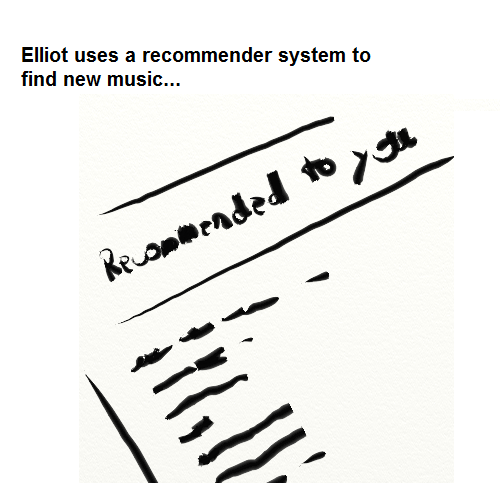
\includegraphics[width=\textwidth]{img/storyboard01}
					\caption{}
					\label{figure:storyboard01}
	\end{subfigure}%
	~
	\begin{subfigure}[t]{0.4\textwidth}
					\centering
					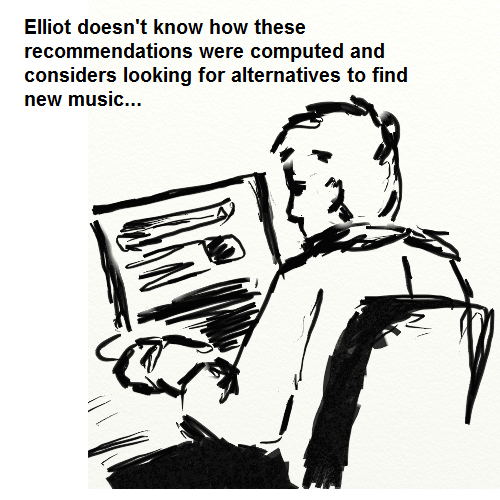
\includegraphics[width=\textwidth]{img/storyboard02}
					\caption{}
					\label{figure:storyboard02}
	\end{subfigure}
	~
	\begin{subfigure}[t]{0.4\textwidth}
					\centering
					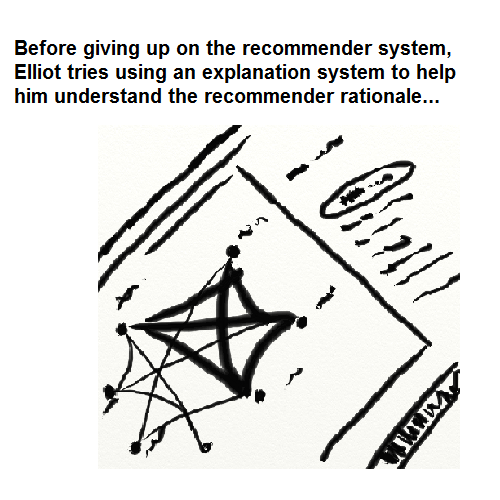
\includegraphics[width=\textwidth]{img/storyboard03}
					\caption{}
					\label{figure:storyboard03}
	\end{subfigure}
	~
	\begin{subfigure}[t]{0.4\textwidth}
					\centering
					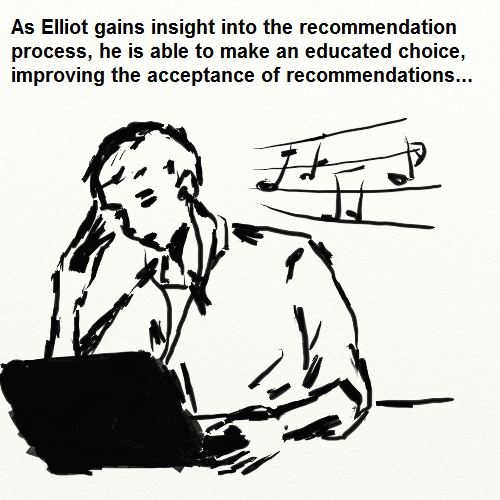
\includegraphics[width=\textwidth]{img/storyboard04}
					\caption{}
					\label{figure:storyboard04}
	\end{subfigure}
	\caption{A selection of the screens used in the user study with paper prototype.}%
	\label{figure:storyboard}%
\end{figure}




%%%%%%%%%%%%%%%%%%%%%%%%%%%%%%%%%%%%%%%%%%%%%%%%%%%%%%%%%%%%%%%%%%%%%%%%%%%%%%%%%%%%%%%%%%%%%%%%%%%
%%%%%%%%%%%%%%%%%%%%%%											USE CASES													%%%%%%%%%%%%%%%%%%%%%
%%%%%%%%%%%%%%%%%%%%%%%%%%%%%%%%%%%%%%%%%%%%%%%%%%%%%%%%%%%%%%%%%%%%%%%%%%%%%%%%%%%%%%%%%%%%%%%%%%%
\section{Use case diagram}

Based on the discussion in section \ref{chapter:literature_study:section:user:subsection:insight}, four interactions can be identified: hovering of items, hovering of users, clicking of items, and clicking of users. The use case diagram is presented in Figure \ref{fig:use_case_diagram} lists each of these interactions. Tables \ref{tab:use_case1}, \ref{tab:use_case2}, \ref{tab:use_case3}, and \ref{tab:use_case4} in appendix \ref{appendix:use_cases} describe each use case in greater detail.

%%%%%%%%%%%%%%%USE CASE DIAGRAM
\begin{figure}
  \begin{center}
  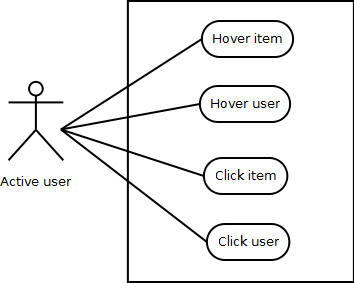
\includegraphics[scale=0.7]{img/usecase_diagram}
	\end{center}
  \caption{Use case diagram of the \emph{SoundSuggest} application.}
  \label{fig:use_case_diagram}
\end{figure}

%\FloatBarrier




